\documentclass[conference, a4paper]{IEEEtran}

\usepackage{graphicx}

% used for flow charts
\usepackage{pgf}
\usepackage{tikz}
\usepackage{tikz-qtree}
\usepackage{reotex}

% package url is used when citing a website
\usepackage{url}

\usepackage{amssymb}
\usepackage{cite}
\usepackage[normalem]{ulem}
% for a smile-face character
\usepackage{wasysym}
% listing for codes
\usepackage{listings}
% listing for golang
% NOTE listings-golang.sty is required
\usepackage{listings-golang}
% to support flow graphs
\usepackage{textcomp}

% positioning is used for below lef = of
\usetikzlibrary{shapes,shadows,arrows,automata,positioning}
% some tikz-styles on reo channels, not required in papers that have nothing to do with Reo

% FIXME finally no todos should exist in this draft
\usepackage[textsize=tiny]{todonotes}

% -------------------------------------- configurations -----------------------------------------
% declaration of environments
\newtheorem{theorem}{Theorem}
\newtheorem{definition}{Definition}
\newtheorem{example}{Example}

% personal characters
\newcommand{\rblock}[0]{\circleddash}
\newcommand{\rread}[0]{\rhd}
\newcommand{\rnoread}[0]{\oslash}
\newcommand{\smap}[1]{[{#1}]}

% style of source code environment listings
\lstset{basicstyle=\footnotesize\ttfamily,breaklines=true, frame=shadowbox}
\lstset{numbers=left}
\lstset{xleftmargin=2em, xrightmargin=2em}
\lstset{language=Golang}

% --------------------------------------- information -------------------------------------------
\title{Active Learning from Blackbox to Timed Connectors}
\author{
\IEEEauthorblockN{Yi Li\IEEEauthorrefmark{1}, Yiwu Wang\IEEEauthorrefmark{1} and Meng Sun\IEEEauthorrefmark{1}}
\IEEEauthorblockA{
\IEEEauthorrefmark{1}Department of Informatics, School of Mathematical Sciences, Peking University,
Beijing, China\\
liyi\_math@pku.edu.cn, yiwuwang@126.com, summeng@math.pku.edu.cn
}
}

\begin{document}
\maketitle
\begin{abstract}
  Coordination models and languages play a key role in formally specifying the communication and
  interaction among different components in large-scale distributed and concurrent systems. In this
  paper, we propose an active learning framework to extract timed connector models from black-box
  system implementation. 
  We first introduce parameterized mealy machine as an operational semantic
  model for channel-based coordination language Reo. Parameterized mealy machine serves as a bridge
  between Reo connectors and mealy machines. With the product operator, complex connectors can be
  constructed by joining basic channels and transformed into mealy machines. Moreover, we adapt L*,
  a well-known learning algorithm, to timed connectors (in the form of mealy machines). The new
  algorithm has shown its efficiency in multiple case studies. 
  Implementations of this framework is provided as a package in \texttt{Golang}.
\end{abstract}

\begin{IEEEkeywords}
  Active Learning, Coordination Languages, Timed Connectors
\end{IEEEkeywords}

\section{Introduction}

Distributed real-time embedded system (DRES) is reforming our lives with the name \emph{IoT}, the
internet of things, wherein systems are usually composed of individual components and a middleware
serving as a \emph{connector}. Such systems could be distributed logically or physically, which
makes the coordination even more complicated. In this case, we need to specify these coordination
processes with so-called \emph{coordination languages}, so that formal techniques can be applied to
guarantee their reliability.

\emph{Timed Reo} is a real-time extension of the coordination language \emph{Reo}. With timeline
involved, coordination process in DRES can be depicted clearly and intuitively. Different formal
semantics are proposed to specify the behavior of timed Reo.
For example, in \cite{DBLP:conf/tase/Meng12}, a UTP-based
(\emph{Unifying Theories of Programming}) semantics is provided to verify connectors as
\emph{designs}. An operational semantics based on \emph{constraint automata} was raised by Baier et
al., where a variant of LTL was also proposed to describe the properties of timed connectors.

Formal verification techniques have also been proved applicable in timed connectors.
\cite{DBLP:conf/tase/LiCWS15} has shown us a comformance testing method on timed connectors.
Bounded model checking methods were also adapted in \cite{DBLP:journals/scp/Kemper12}, based on SAT
solvers. All these solutions seem practical and impressive, however, a common question is faced by
most of them, which is: \emph{How to obtain these formal models?}

\emph{Correctness} of connectors is very much related to some low-level implementation details.
For example, well-writen code may behave dramatically weird with an improper set of concurrency
primitives. Such things happen frequently in embedded systems with different hardware platforms or
operating systems. Consequently, manually modeling an existing connector seems rather unreliable,
even with reference to its source code.

As a branch of \emph{machine learning} technique, active learning offers a way to obtain models from
low-level blackboxes. Works in \cite{DBLP:journals/mt/Daelemans10, DBLP:journals/iandc/Angluin87,
DBLP:conf/fase/RaffeltS06} shows impressive examples where active learning is used to extract
\emph{finite state automatas} or \emph{grammars}. 

\todo{better expressions!}

\begin{figure}[h]
  \begin{center}
    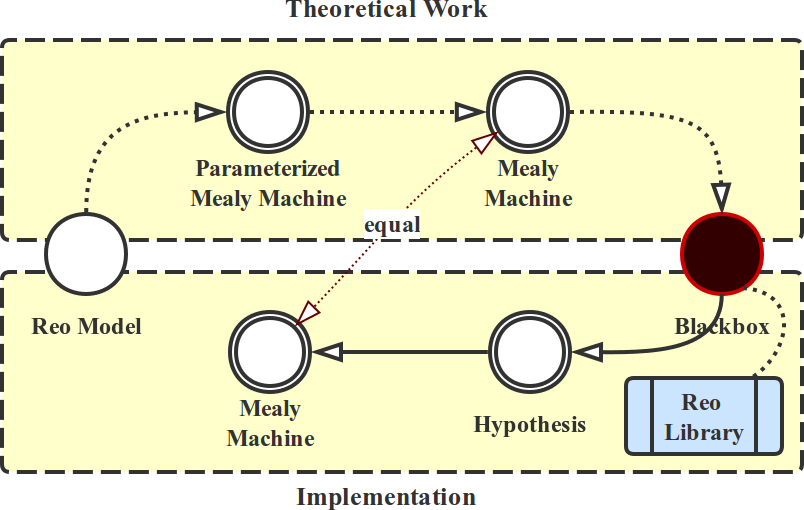
\includegraphics[width=.4\textwidth]{./images/howto.png}
  \end{center}
  \caption{The Active Learning Framework}
  \label{fig:howto}
\end{figure}

In this paper, we proposed a active learning framework (shown in Figure \ref{fig:howto}) to
automatically extract timed connectors from blackbox models. We present \emph{Parameterized Mealy
machine} as a parametierized semantics for timed Reo channels, which enables us to generate Mealy
machines with a given alphabet. Then the $L*$ algorithm is adapted and optimized to extract Mealy
machines with time action from the \emph{connectors in blackboxes}.

The rest of the paper is organized as follows. After this general introduction, in Section
\ref{sec:preliminaries} we briefly illustrate some basic concepts, including Reo the coordination
language, Mealy machine, and active automata learning. Section \ref{sec:semantics} defines the
Mealy-machine-based operational semantics of Reo, which is used in Section \ref{sec:activelearning}
to show how to extract Reo models from blackboxes by means of active learning. Finally, in Section
\ref{sec:experiment}, we discuss the optimization and implementation in \texttt{Golang}.

\section{Preliminaries} 
\label{sec:preliminaries}
\subsection{Reo Coordination Language} 
\label{sec:reo}
We provide here a brief overview of the main concepts of Reo, more details can be found in
\cite{DBLP:journals/mscs/Arbab04, DBLP:journals/scp/BaierSAR06}.

Reo is a channel based exogenous coordination language proposed by F. Arbab in
\cite{DBLP:journals/mscs/Arbab04}. 
A Reo model, also called \emph{connector}, provides the protocol
that formalizes the communication, synchronization and cooperation among the components which
communicate through the connector. Connectors can be defined with no knowledge of the components,
which makes Reo a powerful ``glue language'' in component-based
development\cite{DBLP:journals/sigsoft/Gill03}.

In Reo, complex connectors are made up of simpler ones, where the atomic connectors are called
\emph{channels}. Each channel has two \emph{channel ends}. There are two type of channel ends:
\emph{source} and \emph{sink}. Source channel ends accepts data into the channel, while sink
channels ends release them out of the channel. 

\begin{figure}[h]
  \begin{center}
    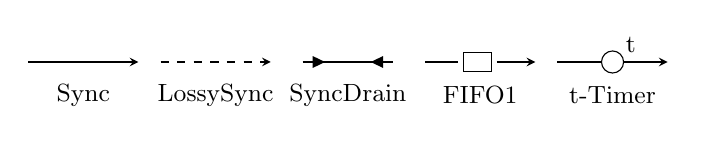
\begin{tikzpicture}[scale=1.4]

\tikzstyle{every node}=[font=\small]
\tikzstyle{label}=[draw=none]

\draw (0.5, -0.3) node[label] {Sync};
\draw (1.7, -0.3) node[label] {LossySync};
\draw (2.9, -0.3) node[label] {SyncDrain};
\draw (4.1, -0.3) node[label] {FIFO1};
\draw (5.3, -0.3) node[label] {t-Timer};

\sync{(0,0)}{(1,0)}{}
\lossysync{(1.2,0)}{(2.2,0)}{}
\syncdrain{(2.4,0)}{(3.4,0)}{}
\fifoe{(3.6,0)}{(4.6,0)}{}

\timer{(4.8,0)}{(5.8,0)}{node [above left] {t}}

\end{tikzpicture}

  \end{center}
  \caption{Basic Reo Channels}
  \label{fig:basic}
\end{figure}

The behavior of some channels are informally described as follows. (Graphical representations
can be found in Figure \ref{fig:basic}).

\begin{itemize}
  \item [-] A \emph{Sync} channel accepts a data item from its source end iff. the data item can be
    dispensed to its sink end simultaneously.
  \item [-] A \emph{LossySync} channel is always prepared to accept data items. These items will be
    send to its sink end simutaneously if possible, otherwise they will be dropped.
  \item [-] A \emph{SyncDrain} channel has two source ends and no sink end. It can accept a data
    item through one of its source end iff. a data item is also available for it to simultaneously
    accept through the other end. Then both two data items will be lost.
  \item [-] A A \emph{FIFO1} channel is an asychronous channel with one buffer cell. It accepts a
    data item whenever the buffer is empty.  
\end{itemize}

Channels are attached on component instances or \emph{nodes}. There are three types of nodes:
\emph{source}, \emph{sink} and \emph{mixed node}, depending on whether all channel ends that
coincide on a node are source ends, sink ends or both. (see in Figure \ref{fig:node})

\begin{figure}[h]
  \begin{center}
    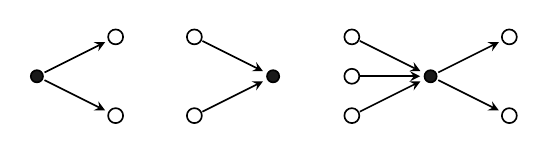
\begin{tikzpicture}[->,>=stealth',shorten >=1pt,auto,node distance=1.6cm,
  semithick]
  \tikzstyle{every node}=[font=\small]

  % source node
  \mixednode{(P-1)}{(-4,0)}{}
  \ionode{(P-2)}{(-3,0.5)}{}
  \ionode{(P-3)}{(-3,-0.5)}{}
  \sync{(P-1)}{(P-2)}{}
  \sync{(P-1)}{(P-3)}{}

  % sink node
  \mixednode{(S-1)}{(-1,0)}{}
  \ionode{(S-2)}{(-2,0.5)}{}
  \ionode{(S-3)}{(-2,-0.5)}{}
  \sync{(S-2)}{(S-1)}{}
  \sync{(S-3)}{(S-1)}{}

  % mixed node
  \ionode{(M-1)}{(0,0.5)}{}
  \ionode{(M-2)}{(0,0)}{}
  \ionode{(M-3)}{(0,-0.5)}{}
  \mixednode{(M-4)}{(1,0)}{}
  \ionode{(M-5)}{(2,0.5)}{}
  \ionode{(M-7)}{(2,-0.5)}{}
  \sync{(M-1)}{(M-4)}{}
  \sync{(M-2)}{(M-4)}{}
  \sync{(M-3)}{(M-4)}{}
  \sync{(M-4)}{(M-5)}{}
  \sync{(M-4)}{(M-7)}{}

\end{tikzpicture}

  \end{center}
  \caption{Source, Sink and Mixed Nodes in Reo}
  \label{fig:node}
\end{figure}



With definition of more basic channels, it's easy to extend Reo to formalize coordination in
different areas. In this paper, we take timed Reo\cite{DBLP:conf/sefm/ArbabBBR04} as our formal
model. Timed Reo includes several timed channels, where the most commonly-used one, called
\emph{timer}, is also shown in Figure \ref{fig:basic}. A t-timer channel accepts any data item from
its source end and returns on its sink end a timeout signal after a delay of t time units.

Components can be linked to source nodes or sink nodes. A component can write data items to its
corresponding source node only if the data item can be dispensed simultaneously to all source ends
on this node. Meanwhile, a component can read a data item only if there is at least one readable
sink end on its corresponding node. A mixed node non-determinstically selects and takes a data item
from one of its coincident sink channel ends and replicates it into all of its coincident source
channel ends.

\begin{figure}[h]
  \begin{center}
    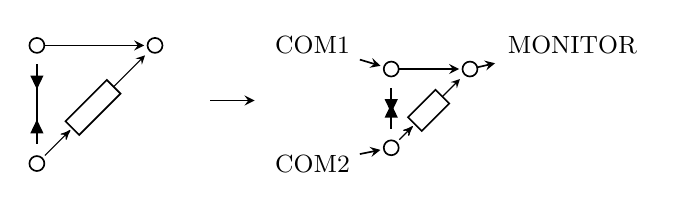
\begin{tikzpicture}[->,>=stealth',shorten >=1pt,auto,node distance=1.6cm,
  semithick]
  \tikzstyle{every node}=[font=\small]

  % draw the alternator
  \ionode{(P-A)}{(0,0)}{}
  \ionode{(P-B)}{(0,-1.5)}{}
  \ionode{(P-C)}{(1.5,0)}{}

  \sync{(P-A)}{(P-C)}{}
  \fifoe{(P-B)}{(P-C)}{}
  \syncdrain{(P-A)}{(P-B)}{}

  % draw the coordination
  \ionode{(C-A)}{(4.5,-0.3)}{}
  \ionode{(C-B)}{(4.5,-1.3)}{}
  \ionode{(C-C)}{(5.5,-0.3)}{}

  \sync{(C-A)}{(C-C)}{}
  \fifoe{(C-B)}{(C-C)}{}
  \syncdrain{(C-A)}{(C-B)}{}

  \node (COM1) at (3.5, 0) {COM1};
  \node (COM2) at (3.5, -1.5) {COM2};
  \node (MONI) at (6.8, 0) {MONITOR};
  \sync{(COM1)}{(C-A)}{}
  \sync{(COM2)}{(C-B)}{}
  \sync{(C-C)}{(MONI)}{}

  \sync{(2.2,-0.7)}{(2.8,-0.7)}{}

\end{tikzpicture}

  \end{center}
  \caption{Coordination with Reo Connectors}
  \label{fig:reoconnector}
\end{figure}

As shown in Figure \ref{fig:reoconnector}, we use a simple example to illustrate how complex
connectors are constructed and used in coordination. In this example, COM1,COM2 and
MONITOR are components. With an \emph{alternator} connector, MONITOR can receive data items from
COM1 and COM2 alternately. The \emph{alternator} example has been implemented in \texttt{Golang} as
shown in Section \ref{sec:reolib}.


\subsection{Mealy Machines}

In this paper, we use \emph{Mealy machine} to model SUTs.
As an extension of \emph{finite state machine}, Mealy machine was first proposed by George. H. Mealy
in \cite{George1955A}. Compared with other variants, Mealy machines are designed to model
reactive systems, where outputs are determined not only by its current state but also the current
inputs. Besides, Mealy machines are supposed to be \emph{input enabled}, which means that all
possible inputs should be acceptable in all states. In other words, if an input is invalid for some
state, we need to manually use an additional state to describe such exceptions.

As far as we can see, various forms of Mealy machines are defined in different works, wherein some
are deterministic and some are not. Since active automata learning very much depends on the
system-under-learn to be deterministic, in this paper we formally define a deterministic version of
Mealy machine following \cite{DBLP:conf/sfm/SteffenHM11}.

\begin{definition}[Mealy machine]
  A Mealy machine is a 6-tuple $(S, s_0, I, O, \delta, \lambda)$ consisting of the following:
  \begin{itemize}
    \item[-] a finite set of states $S$
    \item[-] a start state (also called initial state) $s_0$ which is an element of $S$
    \item[-] a finite set called the input alphabet $I$
    \item[-] a finite set called the output alphabet $O$
    \item[-] a transition function $\delta : S \times I \rightarrow S$ mapping pairs of a
      state and an input symbol to the corresponding next state.
    \item[-] an output function $\lambda : S \times I \rightarrow O$ mapping pairs
      of a state and an input symbol to the corresponding output symbol.
  \end{itemize}
\end{definition}

We say that a Mealy machine is \emph{finite} if the set $S$ of states and the set $I$ of inputs are
finite. Hereinafter, Mealy machines are always supposed to be finite.

A Mealy machine is in some state $q\in S$ is always ready for inputs at any time. If an input symbol
$i\in I$ is provided, the Mealy machine generates output $\lambda(q,i)$ and jumps to state
$\delta(q,i)$.


\subsection{Active Learning}
In this section, we briefly introduce the main ideas of active automata learning. 

Active learning \cite{settles2010active} is a special case of semi-supervised machine learning where
a learning algorithm is able to interactively query the target systems to obtain the desired outputs
on certain inputs. With such flexibility, active learning makes it able to use targeted and efficient
queries to obtain more accurate models with smaller dataset. 


\begin{figure}[h]
  \begin{center}
    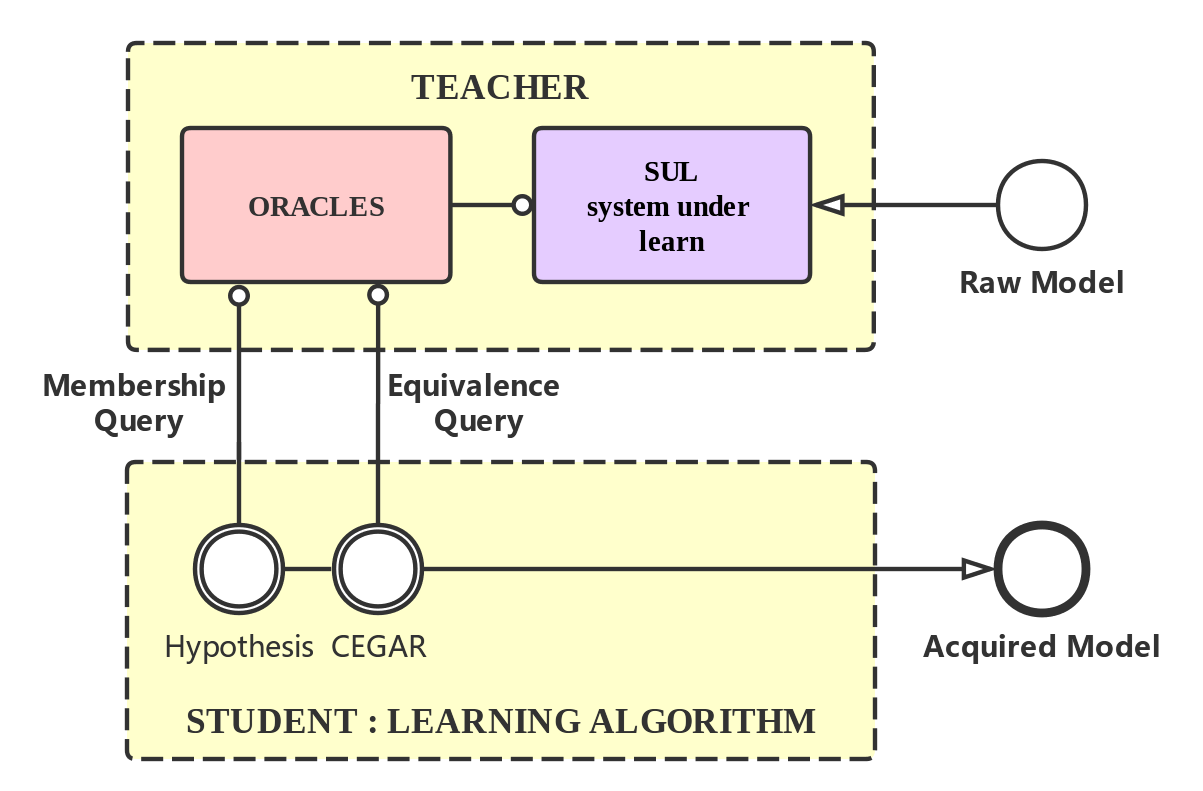
\includegraphics[width=.5\textwidth]{./images/activelearning.png}
  \end{center}
  \caption{Active Automata Learning}
  \label{fig:activelearning}
\end{figure}

Figure \ref{fig:activelearning} shows the sketch of active automata learning, wherein:
\begin{itemize}
  \item[-] \emph{Teacher} and \emph{Student}. Active learning is an interactive process where
    students ask questions and teachers answer. Here learning algorithm plays the role of student.
  \item[-] \emph{Oracles} is an interface specifying which kind of questions can be answered by the
    teacher.
  \item[-] \emph{SUL} is an abbreviation of System Under Learn. The name comes from a well-known
    concept SUT (System Under Test) in software testing. In this case, we use blackbox models as our
    SULs.
  \item[-] \emph{CEGAR} indicates Counter-Example Guided Abstraction
    Refinement\cite{DBLP:conf/cav/ClarkeGJLV00}. In active learning, we need counter-examples to
    guide us on further quries and cover the undistinguished states.
\end{itemize}

When applying active automata learning on some model, firstly we assume that it should be equivalent
to some \emph{Mealy machine}. In other words, a deterministic model accepting a finite set of input
symbols and mapping them to a finite set of output symbols.

Such a model is encapsulated as a \emph{teacher} by the \emph{Oracle}, which handles
all communication with the model, both providing input and obtaining output. Also, it serves as a
so-called \emph{Minimal Adequate Teacher} interface, which is responsible for two types of
queries. 

\begin{itemize}
  \item[-] \textbf{Membership Query} (hereinafter referred to as \emph{mq}) The name comes from
    some grammar-learning papers (e.g. \cite{DBLP:journals/iandc/Angluin87}), where \emph{mq} checks
    if a word is a member of certain language defined by the given grammar. When it comes to
    automata learning, \emph{mq} is supposed to provide \emph{simulation results} for given input
    sequences.
  \item[-] \textbf{Equivalence Query} (hereinaftr referred to as \emph{eq}) Given a hypothesis
    (usually constructed by the learning algorithm), \emph{eq} checks whether the hypothesis is
    equivalent to the system-under-learn and generates a counter-example if needed. Generally, 
    \emph{equivalence query} is irrealizable when SUT is a blackbox. So we tactically use membership
    queries to achieve the approximate results.
\end{itemize}

These queries are given by \emph{learning algorithms}, or so-called \emph{students} in Figure
\ref{fig:activelearning}. From the \emph{mq} results, a learning algorithm should construct a
\emph{hypothesis} and check it with \emph{eq}. If counter-examples are found, we turn back and
repeat the hypothesis construction until the equivalence query returns \emph{true}.

More details on the active automata learning algorithm will be presented in Section
\ref{sec:activelearning}. 

\section{Timed Connectors as Mealy Machines}
\label{sec:semantics}
In this section, we show how a timed connector be transformed into a Mealy machine with time action.

Since time is not involed in original Mealy machine, we first discuss how to formalize the time
dimension in Mealy machine and timed Connectors. After that, we present a \emph{parameterized Mealy
machine} as a bridge between connectors and Mealy machines.

\subsection{Time Domain}
Time is involved in several extension version of Reo. For example, Timed
Reo\cite{DBLP:conf/sefm/ArbabBBR04}, Hybrid Reo\cite{DBLP:conf/icfem/ChenSS14}, etc.
Generally, these models are designed to handle real-time behavior where time is defined in
$\mathbb{R}$. Besides, we also found some works like \cite{DBLP:journals/fmsd/PrabhakarDM015} where
rational time indeed  makes things easier. In this paper, we choose the rational number field
$\mathbb{Q}$ as our time domain, which simplifies discretization of timed behaviors greatly.

As presented in section \ref{sec:reo}, all real-time behavior in timed Reo comes with the
\emph{t-timer} channels, and the number of these channels are apparently finite. We use
$t_i\in\mathbb{Q}$ to denote the delays of these timer channels, and now we can define a precision
function $prec$.
\[
prec(t_1,\cdots,t_n) = \max_T\{\forall t_i.\exists n_i\in\mathbb{N}.t_i=n_i\cdot T\}
\]
It's easy to prove that such a $T$ is always existing.

In real systems, the concept \emph{time precision} is widely used with the name ``clock-period''.
Most of the time, we know the clock-cycle of some hardware components, even without any idea of its
structure. With such precision $T$ given, it's reasonable to assume that all $t$-timers are actually
$nT$-timers. In following sections, we'll use $n$-timers instead.

Besides, we're going to add a ``T'' action in mealy machines. It indicates that a transition
will take a time unit to finish, and all outputs would come out after that.

\subsection{Parameterized Mealy Machine}
We present a model named \emph{parameterized Mealy machine} (hereinafter referred to as PMM)
to represent timed connectors. PMM is supposed to behave as a middle representation. Connectors are
defined as parameterized mealy machines, and composed via its production operator. Then original
mealy-machine model will be taken as semantics of PMM model.

Following the formal definition of Mealy machine in Section \ref{sec:preliminaries}, we present the
definition of \emph{parameterized Mealy machine} as follows.

\begin{definition}[Parameterized Mealy Machine]
  A \emph{Parameterized Mealy Machine} is defined as a 6-tuple $\mathcal{PM}=\langle
  S(\Sigma), s_0, I, O, \delta(\Sigma), \lambda(\Sigma)\rangle$ where 
  \begin{itemize}
    \item[-] $\Sigma$ is a \emph{finite} datum alphabet (hereinafter referred to as an alphabet)
    \item[-] $S$ is a function that maps an alphabet to a \emph{finite} set of
      states. We use $S(\Sigma)$ to denote the state set.
    \item[-] $I$ is a finite set of source-ends.
    \item[-] $O$ is a finite set of sink-ends.
    \item[-] $s_0$ is the initial state. It satisfies $\forall \Sigma,s_0\in S(\Sigma)$
    \item[-] $\delta$ maps a \emph{finite} datum alphabet to an \emph{output function}. We use
      $\delta(\Sigma):S(\Sigma)\times Input(\Sigma,I)\rightarrow Output(\Sigma, O)$ to denote the output function.
    \item[-] $\lambda$ maps an alphabet to a \emph{transition function}. We use
      $\lambda(\Sigma):S(\Sigma)\times Input(\Sigma,I)\rightarrow S(\Sigma)$ to denote the transiton
      function.
  \end{itemize}
\end{definition}

In the definition above, \emph{Input} and \emph{Output} are used to generate a set of input actions
and output actions from the corresponding alphabets and ends. For example, if we have a alphabet
consisting of two items $d_0$ and one source-end named $A$, the input actions would be
\begin{eqnarray*}
  Input(\{d_0\},\{A\}) &=& \{\{A:d_0,B:\rread\},\{A:d_0,B:\rnoread\}, \\
  & & \{A:\bot,B:\rread\},\{A:\bot,B:\rnoread\},T\}
\end{eqnarray*}
where we use $\rread$ to indicate that a end-sink is ready for write, and $\rnoread$ otherwise.

\todo{How to say?}
\[
Input(\Sigma,I)=\{\}\cup\{T\}
\]
where we use $T$ to denote the time action.
\[
Output(\Sigma,I)=\{\}
\]

Parameterized Mealy machines can be seen as an abstract form of Mealy machines, which means that we
still need a convert function between the two models.

\begin{definition}[Concretize Mapping]
  We use $\smap{\mathcal{PM}}_{\Sigma}$ to denote the concrete Mealy machine which is determined by
  an abstract parameterized Mealy machine $\mathcal{PM}$ and the alphabet $\Sigma$. Apparently
  $\smap{\mathcal{PM}}_{\Sigma}$ can be described as
  \begin{eqnarray*}
    \smap{\mathcal{PM}}_{\Sigma} &=& 
    \langle
    \mathcal{PM}.S(\Sigma), \mathcal{PM}.s_0, \\
    & & Input(\Sigma, \mathcal{PM}.I), Output(\Sigma, \mathcal{PM}.O), \\
    & & \mathcal{PM}.\delta(\Sigma), \mathcal{PM}.\lambda(\Sigma),
    \rangle
  \end{eqnarray*}
\end{definition}

Now we can use Parameterized Mealy Machines to define a new semantics for timed Reo. Here we
take one asynchronous channel (FIFO1), one asynchronous channel (Sync) and one timed channel (Timer)
as examples.

\begin{example}[PMM Semantics of FIFO1 channel]
  \label{example:pmmfifo}
  The semantics of FIFO channel with source end $A$ and sink end $B$ can be defined as follows.
  \begin{itemize}
    \item[-] $S(\Sigma)=\{q_0\}\cup\{q_d|d\in\Sigma\}$
    \item[-] $I=\{A\}$, $O=\{B\}$, $s_0=q_0$
    \item[-] output function
      \begin{displaymath}
        \delta(\Sigma)(s,i)=\left\{
        \begin{array}[h]{ll}
          (B:\bot) & s=q_0\land i=(A:\_,B:\rnoread) \\
          (B:d) & s=q_0\land i=(A:d,B:\rread)\\
          \rblock & s=q_0\land i=(A:\bot,B:\rread) \\
          (B:d) & s=q_d\land i=(A:\_,B:\rread)\\
          \rblock & s=q_d\land i=(A:d,B:\rnoread) \\
          (B:\bot) & s=q_d\land i=(A:\_,B:\rnoread) \\     
        \end{array}
        \right.
      \end{displaymath}
    \item[-] transition function
      \begin{displaymath}
        \lambda(\Sigma)(s,i)=\left\{
        \begin{array}[h]{ll}
          q_d & s=q_0\land i=(A:d,B:\rnoread) \\
          q_d & s=q_{d'}\land i=(A:d,B:\rread) \\
          q_0 & otherwise \\
        \end{array}
        \right.
      \end{displaymath}
  \end{itemize}
\end{example}

Besides, the concrete mealy machine (where $\Sigma=\{a\}$) is shown in Figure \ref{fig:pmmfifo}.
\begin{figure}[h]
  \begin{center}
    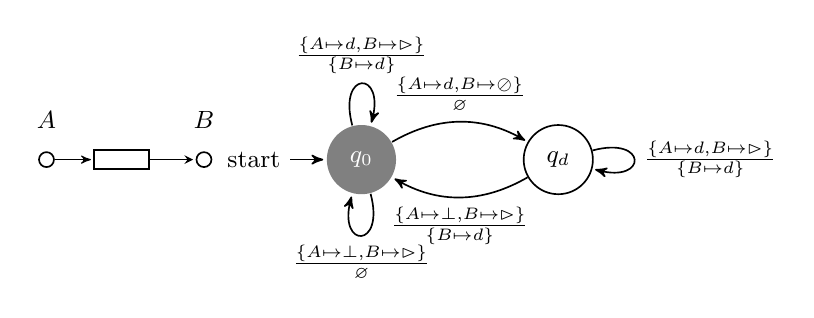
\begin{tikzpicture}[->,>=stealth',shorten >=1pt,auto,node distance=1.6cm,
  semithick]
  \tikzstyle{every node}=[font=\small]
  \ionode{(P-A)}{(-4,0)}{(-4,0.5) node {$A$}}
  \ionode{(P-B)}{(-2,0)}{(-2, 0.5) node {$B$}}
  
  \fifoe{(P-A)}{(P-B)}{}

  \tikzstyle{every state}=[fill=white,text=black,font=\small]
  \tikzstyle{init}=[fill=gray,draw=none,text=white]

  \node[initial,state,init] (Q0)                     {$q_{0}$};
  \node[state]         (QA)  [right = of Q0]    {$q_{d}$};

  \path
  (Q0)
  edge  [bend left]     node {$\frac{\{A\mapsto d, B\mapsto \rnoread\}}{\varnothing}$} (QA)
  edge  [loop below]    node {$\frac{\{A\mapsto \bot, B\mapsto \rread\}}{\varnothing}$} (QA)
  edge  [loop above]    node {$\frac{\{A\mapsto d, B\mapsto \rread\}}{\{B\mapsto d\}}$} (QA)
  (QA)
  edge  [bend left]     node {$\frac{\{A\mapsto \bot,B\mapsto \rread\}}{\{B\mapsto d\}}$} (Q0)
  edge  [loop right]    node {$\frac{\{A\mapsto d,B\mapsto \rread\}}{\{B\mapsto d\}}$} (QA)
  ;
\end{tikzpicture}


  \end{center}
  \caption{PMM-based Semantics of $\smap{FIFO1}_\Sigma$, where $\Sigma=\{a\}$}
  \label{fig:pmmfifo}
\end{figure}

\begin{example}[PMM Semantics of Sync channel]
  The PMM-based semantics of a Sync channel with a source-end A and a sink-end B can be defined as:
  \begin{itemize}
    \item[-] $S(\Sigma)=\{q_0\}$, $I=\{A\}$, $O=\{B\}$, $s_0=q_0$
    \item[-] output function
      \begin{displaymath}
        \delta(\Sigma)(s,i)=\left\{
        \begin{array}[h]{ll}
          (B:\bot) & s=q_0\land i=(A:\bot,B:\rnoread) \\
          (B:d) & s=q_0\land i=(A:d,B:\rread)\\
          \rblock & s=q_0\land i=(A:\bot,B:\rread) \\
          \rblock & s=q_0\land i=(A:d,B:\rnoread) \\
        \end{array}
        \right.
      \end{displaymath}
    \item[-] transition function $\lambda(\Sigma)(s,i)=q_0$.
  \end{itemize}
\end{example}

\begin{example}[PMM Semantics of n-Timer channel]
  Considering a n-Timer channel with a source-end A and a sink-end B, we define its PMM-based
  semantics as:
  \begin{itemize}
    \item[-] $S(\Sigma)=\{q_0\}\cup\{q_d|d\in\Sigma\}$
    \item[-] $I=\{A\}$, $O=\{B\}$, $s_0=q_0$
    \item[-] output function
      \begin{displaymath}
        \delta(\Sigma)(s,i)=\left\{
        \begin{array}[h]{ll}
          (B:\bot) & s=q_0\land i=(A:\_,B:\rnoread) \\
          (B:d) & s=q_0\land i=(A:d,B:\rread)\\
          \rblock & s=q_0\land i=(A:\bot,B:\rread) \\
          (B:d) & s=q_d\land i=(A:\_,B:\rread)\\
          \rblock & s=q_d\land i=(A:d,B:\rnoread) \\
          (B:\bot) & s=q_d\land i=(A:\_,B:\rnoread) \\     
        \end{array}
        \right.
      \end{displaymath}
    \item[-] transition function
      \begin{displaymath}
        \lambda(\Sigma)(s,i)=\left\{
        \begin{array}[h]{ll}
          q_d & s=q_0\land i=(A:d,B:\rnoread) \\
          q_d & s=q_{d'}\land i=(A:d,B:\rread) \\
          q_0 & otherwise \\
        \end{array}
        \right.
      \end{displaymath}
  \end{itemize}
\end{example}

Similarly, we can use parameterized mealy machines to define the semantics of other basic timed Reo
channels. Now we're going to show how to compose these channels into complicated connectors.

\begin{definition}[Production of Parameterized Mealy Machines]
  Now we're going to define the production operator \emph{prod} of two parameterized mealy machines as,
  \[
  prod(PM_1,PM_2)=PM_3
  \]
  as follows. Here we assume that $PM_2.O\cap PM_1.I=\varnothing$
  \begin{itemize}
  	\item[-] $\forall\Sigma, PM_3.S(\Sigma)=PM_1.S(\Sigma)\times PM_2.S(\Sigma)$
    \item[-] $PM_3.I=PM_1.I\cup PM_2.I-PM_1.O$
    \item[-] $PM_3.O=PM_1.O\cup PM_2.O-PM_2.I$
    \item[-] $PM_3.s_0=(PM_1.s_0, PM_2.s_0)$
    \item[-] $\forall\Sigma, PM_3.\delta(\Sigma)((s_1,s_2), i)=$
      \begin{displaymath}
        \left\{
        \begin{array}[h]{ll}
          (Out_1 + Out_2)|_{PM_3.O} & \rblock\land Out_2\neq\rblock \\
          \rblock & otherwise \\
        \end{array}
        \right.
      \end{displaymath}
      where we have
      \begin{itemize}
        \item[*] $In_1 = i|_{PM_1.I}$
        \item[*] $Out_1 = PM_1.\delta(\Sigma)(s_1,In_1)$
        \item[*] $In_2 = (Out_1 + i)|_{PM_2.I}$
        \item[*] $Out_2 = PM_2.\delta(\Sigma)(s_2,In_2)$
      \end{itemize}
    \item[-] $\forall\Sigma, PM_3.\lambda(\Sigma)((s_1,s_2),i)=(s_1',s_2')$
      where we have
      \begin{itemize}
        \item[*] $s_1' = PM_1.\lambda(\Sigma)(s_1,In_1)$
        \item[*] $s_2' = PM_2.\lambda(\Sigma)(s_2,In_2)$
      \end{itemize}
  \end{itemize}
\end{definition}

\todo{example of production, maybe fifo+timer}

\section{From Blackbox to Timed Connectors} 
\label{sec:activelearning}
In this section, we will show how to use L* algorithm to extract models from blackboxes. Firstly, we
presents the definition of \emph{Observation Table}, which is used to describe the hypothesis.

\subsection{Observation Table}

\subsection{Closeness}

\subsection{Counter-Examples}
Generally, equivalence query has been proved impossible in blackbox
models\cite{DBLP:journals/iandc/Angluin87}. However, in this
section, we're showing that in certain circumstances, equivalence query can be implemented with
no approximation.

Equivalence queries are used to search for counter-examples. But what makes counter-examples even
existing? In Reo models, we believe that \emph{FIFO} channels and \emph{Timer} channels are to
blame. Here we present a brief example. To make things eaiser, we have only untimed Reo here.

\begin{figure}[h]
  \begin{center}
    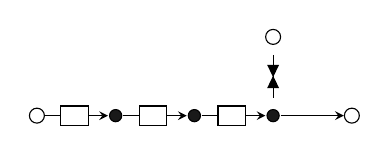
\begin{tikzpicture}

  \ionode{(P-A)}{(0,0)}{}
  \ionode{(P-B)}{(3,1)}{}
  \mixednode{(P-M1)}{(1,0)}{}
  \mixednode{(P-M2)}{(2,0)}{}
  \mixednode{(P-M3)}{(3,0)}{}
  \ionode{(P-C)}{(4,0)}{}

  \fifoe{(P-A)}{(P-M1)}{}
  \fifoe{(P-M1)}{(P-M2)}{}
  \fifoe{(P-M2)}{(P-M3)}{}
  \syncdrain{(P-B)}{(P-M3)}{}
  \sync{(P-M3)}{(P-C)}{}

\end{tikzpicture}

  \end{center}
  \caption{A Switching Connector $S$ with Three Buffers}
  \label{fig:buf3}
\end{figure}

A \emph{Switching} connector in \figurename \ref{fig:buf3} has two source-ends $A,B$ and one
sink-end $C$. In a nutshell, datum come from $A$ and be stored temporarily in buffers. These datum
will never flow out until signals come to $B$. With the Mealy-Machine semantics given, the semantics
of \emph{Switching} connectors can be defined as following \figurename \ref{fig:buf3semantics}.

\begin{figure}[h]
  \begin{center}
    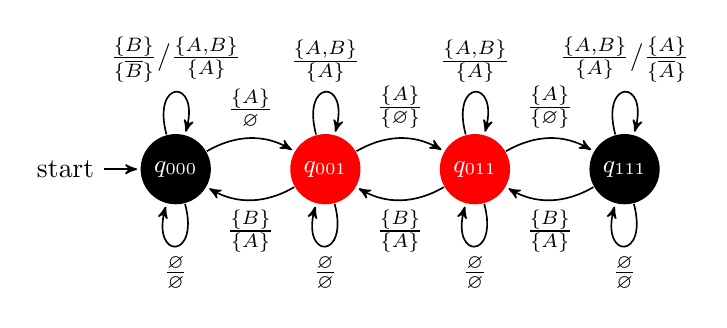
\begin{tikzpicture}[->,>=stealth',shorten >=1pt,auto,node distance=1.9cm,
                    semithick]
  \tikzstyle{every state}=[fill=black,draw=none,text=white,font=\small]
  \tikzstyle{red}=[fill=red]

  \node[initial,state] (Q000)                    {$q_{000}$};
  \node[state,red]         (Q001) [right of=Q000] {$q_{001}$};
  \node[state,red]         (Q011) [right of=Q001] {$q_{011}$};
  \node[state]         (Q111) [right of=Q011] {$q_{111}$};

  \path (Q000) edge  [bend left]   node {$\frac{\{A\}}{\varnothing}$} (Q001)
               edge  [loop below]  node {$\frac{\varnothing}{\varnothing}$} (Q001)
               edge  [loop above]  node {$
                                     \frac{\{B\}}{\{\overline{B}\}}/
                                     \frac{\{A,B\}}{\{A\}}
                                   $} (Q000)
        (Q001) edge  [bend left]   node {$\frac{\{B\}}{\{A\}}$} (Q000)
               edge  [loop below]  node {$\frac{\varnothing}{\varnothing}$} (Q001)
               edge  [loop above]  node {$
                                     \frac{\{A,B\}}{\{A\}}
                                   $} (Q001)
               edge  [bend left]   node {$\frac{\{A\}}{\{\varnothing\}}$} (Q011)
        (Q011) edge  [bend left]   node {$\frac{\{B\}}{\{A\}}$} (Q001)
               edge  [loop below]  node {$\frac{\varnothing}{\varnothing}$} (Q011)
               edge  [loop above]  node {$
                                     \frac{\{A,B\}}{\{A\}}
                                   $} (Q011)
               edge  [bend left]   node {$\frac{\{A\}}{\{\varnothing\}}$} (Q111)
        (Q111) edge  [bend left]   node {$\frac{\{B\}}{\{A\}}$} (Q011)
               edge  [loop below]  node {$\frac{\varnothing}{\varnothing}$} (Q111)
               edge  [loop above]  node {$
                                     \frac{\{A,B\}}{\{A\}}/
                                     \frac{\{A\}}{\{\overline{A}\}}
                                   $} (Q111)
        %(B) edge [loop above] node {1,1,L} (B)
            %edge              node {0,1,L} (C)
        %(C) edge              node {0,1,L} (D)
            %edge [bend left]  node {1,0,R} (E)
        %(D) edge [loop below] node {1,1,R} (D)
            %edge              node {0,1,R} (A)
  ;
\end{tikzpicture}


  \end{center}
  \caption{\emph{Gate} as Mealy Machine $\mathcal{M}(S)$}
  \label{fig:buf3semantics}
\end{figure}

According to the production of Mealy-Machines, 8 different states should be found in
$\mathcal{M}(S)$. We use $q_{abc}$ to denote them. $q_{001}$ indicates that the last buffer is
filled and others are empty, and $q_{111}$ means that there are no space in any buffer. It's
obvious that some states like $q_{100}$ is unreachable.

We say if two states are \emph{similiar} iff. they have the same output signature.

\begin{theorem}[Bound of Counter-Example]
  \label{the:cebound} Assume that an observation table has already been closed with maximum
  query length \todo{find a better phrase?} $l$. An counter-example of length $l+2$ would be
  found iff. there're possible counter-examples.
\end{theorem}
\begin{IEEEproof}
  Sketch of this proof are shown in several points:
  \begin{enumerate}
    \item Hypothesises are subgraphs of the semantics graph.
    \item Inputs on reverse edges are complementary.
    \item 
  \end{enumerate}
\end{IEEEproof}

\section{Experiments} 
\label{sec:experiment}

Both \emph{Reo Coordination Models} and \emph{Adapted L* Algorithm} are implemented in
Golang\cite{golang}.

Golang (or Google Go) is a rising programming language started by Google Inc. The language is widely
known for its elegant design and impressive efficiency. Moreover, the concurrency model of Golang
comes from CSP\cite{DBLP:books/ph/Hoare85}. As a channel-based model, CSP shares a similar idea with
Reo and makes our implementation much more natural.

We have programmed Reo channels as a new package in Golang. The package is well-written for not only
formal verification but also practical use.

All the following experiments are coded under Golang \emph{1.2.1} and executed on a laptop with 8GB
of RAM and a Core i7-3630 CPU. The source code is available at
\url{https://github.com/liyi-david/reo-learn}.

\subsection{Case Studies}
A simple example of timed connector is presented to show how L* works.
\begin{figure}[h]
  \begin{center}
    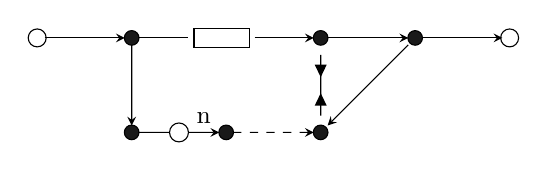
\begin{tikzpicture}[scale=1.2]
  \tikzset{every node} = [font=\small]

  \ionode{(P-A)}{(0,0)}{}
  \ionode{(P-B)}{(5,0)}{}
  \mixednode{(P-C)}{(1,0)}{}
  \mixednode{(P-D)}{(3,0)}{}
  \mixednode{(P-E)}{(4,0)}{}
  \mixednode{(P-F)}{(1,-1)}{}
  \mixednode{(P-G)}{(2,-1)}{}
  \mixednode{(P-H)}{(3,-1)}{}

  \fifoe{(P-C)}{(P-D)}{}
  \syncdrain{(P-D)}{(P-H)}{}
  \sync{(P-A)}{(P-C)}{}
  \sync{(P-C)}{(P-F)}{}
  \sync{(P-D)}{(P-E)}{}
  \sync{(P-E)}{(P-B)}{}
  \sync{(P-E)}{(P-H)}{}
  \lossysync{(P-G)}{(P-H)}{}

  \timer{(P-F)}{(P-G)}{node [above] {n}}

\end{tikzpicture}

  \end{center}
  \caption{Expiring FIFO1 Channel}
  \label{fig:expfifo}
\end{figure}
 
\subsection{Performance Optimization}
As a well-known learning algorithm, L* has proved its efficiency in models without time.
However, when dealing with timed connectors, the algorithm failed to meet our expectation.

\begin{table}[h]
  \renewcommand{\arraystretch}{1.3}
  \caption{Time-Cost Analysis}
  \label{tabel:timecost}
  \centering
  \begin{tabular}{l||rrr}
    \hline
    & FIFO & Alternator & Gate \\
    \hline\hline
    Membership Query(s) & 41.571 & 126.468 & 169.161 \\
    Hypothesis Query(s) & 0.001 & 0.003 & 0.004 \\
    Total Time(s) & 41.715 & 165.114 & 247.098\\
    Membership Query(\%) & 99.6 & 76.6 & 68.5\\
    \hline
  \end{tabular}
\end{table}

As shown in Table \ref{tabel:timecost}, time consumption mainly comes from membership queries.
Since time is involved in our model, it's inevitably that simulation takes time to behave normally.
Even worse, since our models are treated as blackbox. With no access to inner behaviour of the
connectors, it's almost impossible to accelerate the simulation process.

Fortunately, there are still other optimization solutions. After reviewing our algorithm, we found
that simulations on similar sequences were invoked frequently:

\begin{itemize}
  \item When constructing \emph{Obs} tables, there are lots of redundant calls to membership
    queries. For example, a sequence with prefix 'aa' and suffix 'b' is exactly same as another one
    with prefix 'a' and suffix 'ab'.
  \item Simulation on mealy machines can provide multi-step output. Consequently, if we has
    simulated an 'abc' sequence, there's no reason to perform simulation on an 'ab' sequence.
\end{itemize}

If previous simulation results are stored in a well-maintained cache, the time-cost in
simulation process could be reduced signficiantly. In this work, we use a multiway tree to buffer
these results. A brief example of such trees can be found in Figure \ref{fig:multiway}.

\todo{the graph need further details}
\begin{example}[Multiway-Tree Cache]
  \label{example:tree}
  Considering the FIFO channel presented in Example \ref{example:pmmfifo}. 
  \begin{figure}[h]
    \begin{center}
      \begin{tikzpicture}

\tikzset{grow'=right, level distance=42pt}
\tikzset{execute at begin node=\strut}
\tikzset{every tree node/.style={anchor=base west}}

\Tree [.$q_0$ [.$q_0$ [.$q_0$ ... ] [.$q_a$ ] ... ] [.$q_a$ ... ] ]
\end{tikzpicture}

    \end{center}
    \caption{Multiway-Tree Cache}
    \label{fig:multiway}
  \end{figure}
  Note that in this figure, only the edge information is stored. States like $q_0,q_a$ are written
  here only to make it clear.
\end{example}

\begin{table}[h]
  \renewcommand{\arraystretch}{1.3}
  \caption{Reduction of Membership Queries}
  \label{tabel:cacheoptimization}
  \centering
  \begin{tabular}{l||rrr}
    \hline
    & FIFO & Alternator & Gate \\
    \hline\hline
    Original Algorithm & 93 & 880 & 1034 \\
    Cached Algorithm & 90 & 725 & 707 \\
    Reduction Rate & 3.2\% & 21.4\% & 31.6\% \\
    \hline
  \end{tabular}
\end{table}

With cache applied, we have made a good reduction on the calls of membership queries. The results
can be found in Table \ref{tabel:cacheoptimization}.

\subsection{An Example of the Reo Package }
\label{sec:reolib}

As mentioned above, our implementation in \texttt{Golang} is well-prepared not only for academic use
but also for practical concurrent programming. The following code shows how to compose an alternator
connector (see Figure \ref{fig:reoconnector}) in \texttt{Golang}. An intact version of this example can be found in our github repo.

\begin{lstlisting}
package main

import . './lib/reo'

func alternator(A, B, C Port) {
  // definition of ports
  M0 := MakePort()
  // M1 ... M5 defined similarly

  // definition of channels
  /* NOTE
  go function() means that the function would
  be executed as a new parallel task
  */
  go ReplicatorChannel(A, M0, M1)
  go ReplicatorChannel(B, M2, M3)
  go MergerChannel(M4, M5, C)

  go SyncdrainChannel(M1, M2)
  go SyncChannel(M0, M4)
  go FifoChannel(M3, M5)
}
\end{lstlisting}

Provided with the source and sink nodes, \emph{alternator} function creates a series of basic
channels and mixed nodes (named \emph{Port}) to serve as the alternator connector we need. Now we
can activate the components and using \emph{alternator} function to coordinate them.

\begin{lstlisting}
A := MakePort()
B := MakePort()
C := MakePort()
alternator(A, B, C)

go sender(A, "MSG A")
go sender(B, "MSG B")
go monitor(C)
\end{lstlisting}

In this case, \emph{sender} are goroutines (basic parallel units in \texttt{Golang}) that keep
sending certain messages to some given port (A and B). A \emph{monitor} keep trying to read data
items from the sink end C and print them on the screen. Finally we have a interleaved sequence of
``MSG\_A'' and ``MSG\_B''.
 
\section{Conclusion and Future Work}
Future work should focus on better representation on timed connectors and implementation of
equivanlence query.

\bibliographystyle{abbrv}
\bibliography{bib}

% FIXME remove this
\listoftodos

\end{document}
